\documentclass{subfiles}
\begin{document}
\begin{figure}[!h]
    \centering
    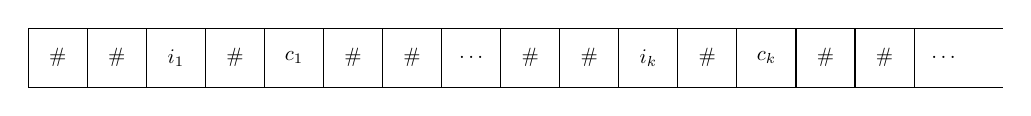
\begin{tikzpicture}[scale = 0.75, every node/.style={scale = 0.75}]

        \draw (-8, 0) -- (-8, -1)
        (-8, 0) -- (8.5, 0)
        (-8, -1) -- (8.5, -1);

        \foreach \i in {-7, -6, ..., 7} {
                \draw (\i, 0) -- (\i, -1);
            }

        \foreach \i in {-8, -7, -5, -3, -2, 0, 1, 3, 5, 6} {

                \node [] () at (\i + 0.5, -0.5) {\#};
            }

        \node [] () at (-5.5, -0.5) {\(i_{1}\)};
        \node [] () at (-3.5, -0.5) {\(c_{1}\)};
        \node [] () at (-0.5, -0.5) {\(\ldots\)};
        \node [] () at (2.5, -0.5) {\(i_{k}\)};
        \node [] () at (4.5, -0.5) {\(c_{k}\)};
        \node [] () at (7.5, -0.5) {\(\ldots\)};

    \end{tikzpicture}
    \caption{MT simulante RAM con costo logaritmico.}
    \label{Fig:3}
\end{figure}
\end{document}